\documentclass{article}

\usepackage[sans, stdmargin, noindent]{../../rajeev}
\usepackage{listings}
\usepackage{graphicx}
\usepackage{animate}

\lstset{style=mystyle}

\pagestyle{fancy}
\rhead{\today}
\lhead{Math 291H Computational Lab \#2}

\begin{document}

\begin{center}
    \Large \textbf{Math 291H Computational Lab \#2}
\end{center}
  
\begin{center}
    \Large Rajeev Atla
\end{center}


\problem{1}
We use Python 3 for this lab, especially the SymPy package.
\lstinputlisting[language=Python, firstline=1, lastline=15]{test1.py}

\problem{2}
\lstinputlisting[language=Python, firstline=18, lastline=47]{test1.py}

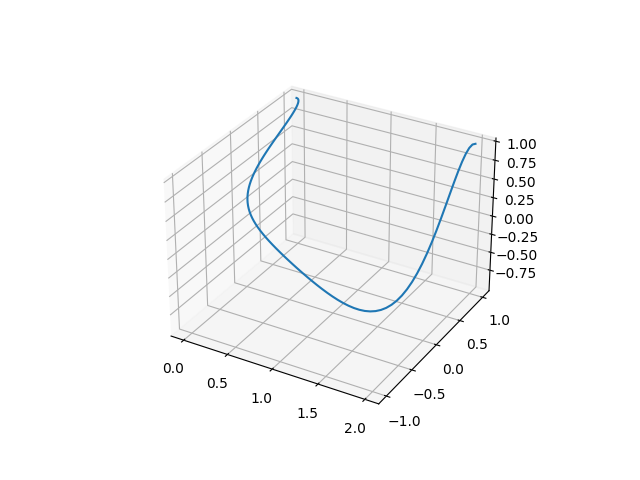
\includegraphics{fig1.png}

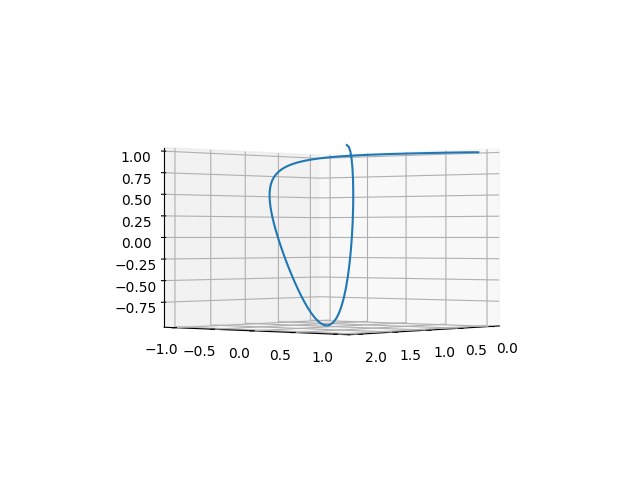
\includegraphics{fig2.png}


\problem{3}
\lstinputlisting[language=Python, firstline=51, lastline=73]{test1.py}

\animategraphics{33}{fig3-}{0}{99}


\problem{4}
\lstinputlisting[language=Python, firstline=77, lastline=84]{test1.py}

The length of the curve is $\approx 6.913$.

\problem{5}
\lstinputlisting[language=Python, firstline=88, lastline=99]{test1.py}

\begin{align*}
  \bm{T} \pars{0} &= \bm{e}_1 \\
  \bm{T} \pars{\frac{T_f}{2}} & \approx 0.515 \bm{e}_1 - 0.857 \bm{e}_2 \\
  \bm{T} \pars{T_f} &= \bm{e}_1 \\
\end{align*}

\problem{6}
\lstinputlisting[language=Python, firstline=103, lastline=111]{test1.py}

\begin{align*}
  \bm{N} \pars{0} &= - \bm{e}_2 \\
  \bm{N} \pars{\frac{T_f}{2}} & \approx - 0.272 \bm{e}_1 + 0.948 \bm{e}_2 - 0.164 \bm{e}_3 \\
  \bm{N} \pars{T_f} &= - \frac{\sqrt{82}}{82} \bm{e}_2 - \frac{9 \sqrt{82}}{82} \bm{e}_3 \\
\end{align*}

\problem{7}
\lstinputlisting[language=Python, firstline=103, lastline=111]{test1.py}

\begin{align*}
  \bm{B} \pars{0} &= - \bm{e}_3 \\
  \bm{B} \pars{\frac{T_f}{2}} &= 0.813 \bm{e}_1 + 0.318 \bm{e}_2 + 0.488 \bm{e}_3 \\
  \bm{B} \pars{T_f} & \approx \frac{9 \sqrt{82}}{82} \bm{e}_2 - \frac{\sqrt{82}}{82} \bm{e}_3 \\
\end{align*}


\problem{8}
\lstinputlisting[language=Python, firstline=123, lastline=145]{test1.py}

\animategraphics{33}{fig4-}{0}{98}

\problem{9}
\lstinputlisting[language=Python, firstline=148, lastline=151]{test1.py}


\begin{align*}
  \kappa \pars{0} &= 4 \pi^2 \\
  \kappa \pars{\frac{T_f}{2}} & \approx 2.757  \\
  \kappa \pars{T_f} &= \frac{4 \pi^2 \sqrt{82}}{9}\\
\end{align*}
\end{document}



